\subsection{关于向量测度的向量值函数的积分}

命题 11. --- 设 F、G、H 为三个 Banach 空间， \(\Phi\) 为 F × G 到 H 中的连续双线性映射。设 m 为 T 上取值于 G 的可优超向量测度。则存在唯一的连续线性映射 I \(_{\Phi,\mathbf{m}}\) （由 \(\overline{\mathcal{L}}_{\mathrm{F}}^{1}(|\mathbf{m}|)\) 到 H 中），使得对每个 z ∈ F 与每个关于 \textbar m\textbar 可积的数值函数 h ，有 I \(_{\Phi,\mathbf{m}}(hz) = \Phi(z, \int h dm)\) 。此外，

\[
\left| \mathrm{I} _ {\Phi , \mathbf {m}} (\mathbf {f}) \right| \leqslant \| \Phi \| \int | \mathbf {f} | d | \mathbf {m} |\tag{4}
\]

对每个函数 \(\mathbf{f} \in \overline{\mathcal{L}}_{\mathrm{F}}^{1}(|\mathbf{m}|)\) 成立。

若存在这样的映射，它对 \(\mathbf{f}\) （ \(|\mathbf{m}|\) -可积集上的阶梯函数）所取的值就被唯一确定：因为已知这时可以写 \(\mathbf{f} = \sum_{i} \mathbf{a}_{i} \varphi_{\mathrm{X}_{i}}\) ，其中诸 \(\mathrm{X}_{i}\) 是 \(|\mathbf{m}|\) -可积且两两不相交的，而诸 \(\mathbf{a}_{i} \in \mathrm{F}\) （Ch. IV, §4, No.~9, 引理）。于是 \(\mathrm{I}_{\Phi, \mathbf{m}}(\mathbf{f})\) 的值就必须等于 \(\sum_{i} \Phi(\mathbf{a}_{i}, \int \varphi_{\mathrm{X}_{i}} d\mathbf{m})\) 。而今，我们有（No.~3, 命题 5）

\[
\left| \sum_ {i} \Phi (\mathbf {a} _ {i}, \int \varphi_ {\mathrm{X} _ {i}} d \mathbf {m}) \right| \leqslant \| \Phi \| \cdot \sum_ {i} | \mathbf {a} _ {i} | \cdot | \mathbf {m} | (\mathrm{X} _ {i}) = \| \Phi \| \int | \mathbf {f} | d | \mathbf {m} |,\tag{5}
\]

这首先表明 H 的元素 \(\sum_{i} \Phi(a_i, \int \varphi_{X_i} d\mathbf{m})\) 不依赖于 \(\mathbf{f}\) 写成 \(\sum_{i} a_i \varphi_{X_i}\) 的特殊形式，因此可以把它记作 \(I_{\Phi, \mathbf{m}}(\mathbf{f})\) 。立即可以验证，如此定义的映射 \(I_{\Phi, \mathbf{m}}\) 在空间 \(\mathcal{E}_F\) （由 \(|\mathbf{m}|\) -可积集上的阶梯函数组成的空间）上是线性的：因为，只需把两个函数 \(\mathbf{f}, \mathbf{g}\) （ \(\mathcal{E}_F\) 中的函数）写成 \(\mathbf{f} = \sum_{i} a_i \varphi_{X_i}\) 与 \(\mathbf{g} = \sum_{i} b_i \varphi_{X_i}\) 的形式，其中诸 \(|\mathbf{m}|\) -可积集 \(X_i\) 作成一个两两不相交的有限族（根据 Ch. IV, §4, No.~9 的引理，这是可能的）。于是不等式 (5) 表明 \(I_{\Phi, \mathbf{m}}\) 在 \(\mathcal{E}_F\) 上连续，而由于这个子空间在 \(\overline{\mathscr{L}}_F^1\) 中稠密（Ch. IV, §4, No.~10, 命题 19 的推论 1 以及 Ch. V, §1, No.~3），由此即得 \(I_{\Phi,m}\) 的存在性与唯一性，以及不等式 (4)。

我们把 \(I_{\Phi,\mathbf{m}}(\mathbf{f})\) 称为 f 关于 m 的积分（相对于双线性映射 \(\Phi\) ）；当双线性映射 \(\Phi\) 在点 \((\mathbf{x},\mathbf{y})\) 处的值记作 xy 时，我们将用 \(\int f dm\) 代替 \(I_{\Phi,\mathbf{m}}(\mathbf{f})\) 。

采用第 6 目的记号，积分 \(\int \langle \mathbf{f},\mathbf{g}\rangle d\mu\) 不是别的，正是 \(\mathrm{I}_{\Phi ,\mathbf{m}}(\mathbf{f})\) （取 \(\Phi (\mathbf{x},\mathbf{x}^{\prime}) = \langle \mathbf{x},\mathbf{x}^{\prime}\rangle\) 与 \(\mathbf{m} = \mathbf{g}\cdot \mu\) ）

推论. --- 若 m 与 \(m'\) 是 T 上取值于 G 的两个可优超测度，则 \(I_{\Phi,m+m'} = I_{\Phi,m} + I_{\Phi,m'}\) ，并且 \(I_{\Phi,\lambda m} = \lambda I_{\Phi,m}\) （对每个标量 \(\lambda\) ）。

第二个断言是直接的。第一个断言的意思是，对每个既 \(|m|\) -可积又 \(|m'|\) -可积的函数 f，

\[
\mathrm{I} _ {\Phi , \mathbf {m} + \mathbf {m} ^ {\prime}} (\mathbf {f}) = \mathrm{I} _ {\Phi , \mathbf {m}} (\mathbf {f}) + \mathrm{I} _ {\Phi , \mathbf {m} ^ {\prime}} (\mathbf {f}).\tag{6}
\]

函数 \(\mathbf{f}\) 是 \((|\mathbf{m}| + |\mathbf{m}'|)\) -可积的（Ch. V, §2, No.~2, 命题 3 的推论 1），从而更是 \((|\mathbf{m} + \mathbf{m}'|)\) -可积的，于是 (6) 的第一端确实有意义。为证明 (6)，只需对 \(\mathbf{f}\) 是 \((|\mathbf{m}| + |\mathbf{m}'|)\) -可积集上的阶梯函数的情形加以证明，因为这些函数所成之集在 \(\overline{\mathcal{L}}_{\mathrm{F}}^{1}(|\mathbf{m}| + |\mathbf{m}'|)\) 中稠密，且由 (4)，(6) 的两端在该空间中都连续。而对 \(\mathbf{f} = \mathbf{a}\varphi_{\mathrm{X}}\) （其中 \(\mathrm{X}\) 是 \((|\mathbf{m}| + |\mathbf{m}'|)\) -可积的），(6) 的两端都化为 \(\Phi(\mathbf{a}, \int \varphi_{\mathrm{X}} d\mathbf{m}) + \Phi(\mathbf{a}, \int \varphi_{\mathrm{X}} d\mathbf{m}')\) ，由此即得推论。

注记. --- 当 \(\mathbf{m}\) 具有形式 \(\mathbf{b}\mu\) （其中 \(\mathbf{b} \in G\) ， \(\mu\) 是 \(T\) 上的实测度）时，

\[
\mathrm{I} _ {\Phi , \mathbf {m}} (\mathbf {f}) = \int \Phi (\mathbf {f} (t), \mathbf {b}) d \mu (t)
\]

对每个函数 \(\mathbf{f} \in \mathcal{L}_{\mathrm{F}}^{1}(\mu)\) 成立，因为两端在该空间上连续，且当 \(\mathbf{f}\) 是 \(|\mu|\) -可积集上的阶梯函数时它们一致。

\subsection{复测度}

定义 6. --- 把复向量空间 \(\mathcal{K}_{\mathbf{C}}(\mathrm{T})\) 上的每个连续线性形式都称为 T 上的复测度。 \(^{2}\)

于是，T 上复测度所成的空间 \(\mathcal{M}_{\mathbf{C}}(\mathrm{T})\) 就是 Hausdorff 局部凸空间 \(\mathcal{K}_{\mathbf{C}}(\mathrm{T})\) 的对偶。

若 \(m\) 是 \(\mathrm{T}\) 上的复测度，它在 \(\mathcal{H}(\mathrm{T})\) 上的限制是 \(\mathrm{T}\) 上取值于 \(\mathbf{C}\) 的向量测度（看作 \(\mathbf{R}\) 上的向量空间）；

m 由这一限制确定，因为若 \(f = f_{1} + if_{2} \in \mathcal{K}_{\mathbf{C}}(\mathrm{T})\) ，则 f 的实部 \(f_{1}\) 与虚部 \(f_{2}\) 都属于 \(\mathcal{K}(\mathrm{T})\) ，且 \(m(f) = m(f_{1}) + im(f_{2})\) 。反过来，对 T 上取值于 C 的每个向量测度 \(m_{0}\) ，公式 \(m(f) = m_{0}(f_{1}) + im_{0}(f_{2})\) 定义一个复测度 m，它是 T 上唯一的在 \(\mathcal{K}(\mathrm{T})\) 上的限制等于 \(m_{0}\) 的测度。因此，今后我们把复测度与它在 \(\mathcal{K}(\mathrm{T})\) 上的限制等同起来；这样的测度 m 具有形式 \(m = \mu_{1} + i\mu_{2}\) ，其中 \(\mu_{1}\) 与 \(\mu_{2}\) 是 T 上的两个实测度，分别称为 m 的实部与虚部。m 的支集是 \(\mu_{1}\) 与 \(\mu_{2}\) 的支集的并。已知 m 是可优超的（No.~3, 命题 4 的推论）；我们把正测度 \(|m|\) 称为 m 的绝对值，它对应于 C 上的绝对值 \(|x_{1} + ix_{2}| = \sqrt{x_{1}^{2} + x_{2}^{2}}\) 。我们有 \(|m| = (\mu_{1}^{2} + \mu_{2}^{2})^{1/2}\) （No.~4, 命题 9 之后的注记）, \(^{3}\) 以及 \(|\mu_{1}| \leqslant |m|\) ， \(|\mu_{2}| \leqslant |m|\) ， \(|m| \leqslant |\mu_{1}| + |\mu_{2}|\) ；此外，m 是以 \(|m|\) 为基的测度，且可写 \(m = h \cdot |m|\) ，其中 \(h \in \mathcal{L}_{\mathbf{C}}^{\infty}(|m|)\) ，且 \(|h(t)| = 1\) 关于 \(|m|\) 局部几乎处处成立（No.~4, 命题 9）。 \(^{4}\) m 与 \(|m|\) 的支集相同。

对每个映射 \(\mathbf{f}\) （由 \(\mathrm{T}\) 到复 Banach 空间 \(\mathbf{F}\) 中的映射，关于 \(|m|\) 本质可积），可以定义（No.~7） \(\mathbf{f}\) 关于 \(m\) 的积分（对应于 \(\mathbf{R}\) -双线性映射 \((\mathbf{x},\lambda)\mapsto\lambda\mathbf{x}\) ，由 \(\mathbf{F}\times\mathbf{C}\) 到 \(\mathbf{F}\) 中），把它记作 \(\int\mathbf{f}dm\) ；由命题 11 的唯一性性质立即得出（采用前面的记号） \(\int\mathbf{f}dm=\int\mathbf{f}d\mu_{1}+i\int\mathbf{f}d\mu_{2}=\int\mathbf{f}hd|m|\) 。因此有 \(m(f)=\int fdm\) （对 \(f\in\mathcal{H}_{\mathbf{C}}(\mathrm{T})\) ）。我们说 \(\mathbf{f}\) 关于 \(m\) 本质可积，意思就是它关于 \(|m|;^{5}\) 本质可积； \(m\) -可积、 \(m\) -可测、局部 \(m\) -可积、 \(m\) -可忽略或局部 \(m\) -可忽略的映射都类似地定义。我们写

\[
\mathcal {L} _ {\mathrm{F}} ^ {p} (\mathrm{T}, m) \left(\mathrm{resp.} \overline {{\mathcal {L}}} _ {\mathrm{F}} ^ {p} (\mathrm{T}, m), \mathrm{L} _ {\mathrm{F}} ^ {p} (T, m)\right)
\]

代替 \(\mathcal{L}_{\mathrm{F}}^{p}(\mathrm{T},|m|)\) （相应地， \(\overline{\mathcal{L}}_{\mathrm{F}}^{p}(\mathrm{T},|m|)\) ， \(\mathrm{L}_{\mathrm{F}}^{p}(\mathrm{T},|m|)\) ）；它们都是复向量空间。

为使 f 为 m-可积（相应地，本质 m-可积），必须且只需 f 关于四个测度 \(\mu_{1}^{+}, \mu_{1}^{-}, \mu_{2}^{+}, \mu_{2}^{-}\) 中的每一个都可积（相应地，本质可积），这要依据 \(|m|, |\mu_{1}|, |\mu_{2}|\) 之间的诸不等式以及关系式 \(|\mu_{k}| = \mu_{k}^{+} + \mu_{k}^{-}\) （Ch. V, §2, No.~2, 命题 3 及其推论 1）。

若 f 本质 m-可积（相应地，m-可积），则 \(|f|\) 本质 \(|m|\) -可积（相应地， \(|m|\) -可积），且由命题 11 得出

\[
\left| \int \mathbf {f} d m \right| \leqslant \int | \mathbf {f} | d | m |.\tag{7}
\]

设 F 与 G 为两个复 Banach 空间，u 为 F 到 G 中的连续线性映射。若 f 是 T 到 F 中的本质 m-可积（相应地，m-可积）映射，则 \(u \circ f\) 本质 m-可积（相应地，m-可积），且 \(\int(u \circ f) dm = u (\int f dm)\) ；这由前文以及关于本质 \(|m|\) -可积函数的类似命题立即得出（Ch. IV, §4, No.~2, 定理 1 以及 Ch. V, §1, No.~3, 引理与定义 3）。

设 \(m\) 是 \(T\) 上的复测度， \(h\) 是局部 \(m\) -可积的复函数。对每个函数 \(f \in \mathcal{K}_{\mathbf{C}}(T)\) ，函数 \(fh\) 是 \(m\) -可积的，且映射 \(f \mapsto \int fh dm\) 是一个复测度，记作 \(h \cdot m\) ，称为以 \(h\) 为密度（关于 \(m\) ）的测度。若 \(m = g \cdot |m|\) ，则显然 \(h \cdot m = hg \cdot |m|\) ；此外，由于 \(|g(t)| = 1\) 关于 \(|m|\) 局部几乎处处成立，为使 \(\mathbf{f}\) 关于 \(n = h \cdot m\) 本质可积，必须且只需 \(\mathbf{f}h\) 本质 \(m\) -可积，且这时有 \(\int \mathbf{f} dn = \int (\mathbf{f}h) dm\) 。此外还有 \(|h \cdot m| = |h| \cdot |m|\) 。我们也把每个形如 \(h \cdot m\) 的测度称为以 \(m\) 为基的复测度；若两个复测度 \(m, m'\) 中的每一个关于另一个都具有密度，亦即 \(m' = h \cdot m\) （其中 \(h\) 局部 \(m\) -可积，且 \(h(t) \neq 0\) 关于 \(|m|\) 局部几乎处处成立），则称这两个复测度等价。显然 \(m\) 与 \(|m|\) 等价，且为使 \(m\) 与 \(m'\) 等价，必须且只需 \(|m|\) 与 \(|m'|\) 等价。

若 m 与 \(m'\) 是 T 上的两个复测度，f 是取值于复 Banach 空间 F 的函数，关于 m 与 \(m'\) 都本质可积（相应地，可积），则对任意复数 \(\lambda\) 与 \(\lambda'\) ，f 关于 \(\lambda m + \lambda'm'\) 本质可积（相应地，可积），且

\[
\int \mathbf {f} d (\lambda m + \lambda^ {\prime} m ^ {\prime}) = \lambda \int \mathbf {f} d m + \lambda^ {\prime} \int \mathbf {f} d m ^ {\prime}.
\]

因为这由第 7 目命题 11 的推论得出。

此外，由定义得出

\[
\left| \lambda m + \lambda^ {\prime} m ^ {\prime} \right| \leqslant \left| \lambda \right| \cdot \left| m \right| + \left| \lambda^ {\prime} \right| \cdot \left| m ^ {\prime} \right|.
\]

我们把复测度 m 的共轭测度称为复测度 \(\overline{m}\) ，它由 \(\overline{m}(f) = \overline{m(\overline{f})}\) （对 \(f \in \mathcal{K}_{\mathbf{C}}(\mathrm{T})\) ）定义。若 \(m = \mu_{1} + i\mu_{2}\) （其中 \(\mu_{1}\) 与 \(\mu_{2}\) 是实测度），则 \(\overline{m} = \mu_{1} - i\mu_{2}\) 且 \(|\overline{m}| = |m|\) ；若 \(m = h \cdot |m|\) ，则 \(\overline{m} = \overline{h} \cdot |m|\) 。若 f 是取复值的本质 m-可积（相应地， \(m\) -可积）函数，则 \(\overline{f}\) 本质 \(\overline{m}\) -可积（相应地， \(\overline{m}\) -可积），且

\[
\int \overline {{f}} d \overline {{m}} = \overline {{\int f d m}}.
\]

命题 12. --- 设 m 是 T 上的复测度，p 与 q 是共轭指数（Ch. IV, §6, No.~4）。双线性型 \((f,g)\mapsto\int fg dm\) 在乘积空间 \(\mathcal{L}_{\mathbf{C}}^{p}(m)\times\mathcal{L}_{\mathbf{C}}^{q}(m)\) 上有定义且连续；不等式 \(\left|\int fg dm\right|\leqslant\mathrm{N}_{p}(f)\mathrm{N}_{q}(g)\) 成立，且 \(\mathrm{N}_{q}(g)\) 是 \(\mathrm{L}_{\mathbf{C}}^{p}(m)\) 上由线性形式 \(f\mapsto\int fg dm\) 通过过渡到商得到的连续线性形式的范数。

此外，若 \(1 \leqslant p < +\infty\) ，则复向量空间 \(\mathcal{L}_{\mathbf{C}}^{p}(m)\) 上的每个连续线性形式都具有 \(f \mapsto \int fg dm\) 的类型，其中 \(g\) 是 \(\mathcal{L}_{\mathbf{C}}^{q}(m)\) 中的一个函数，它在 \(\mathrm{L}_{\mathbf{C}}^{q}(m)\) 中的类被唯一确定。

由于 \(m = h \cdot |m|\) （其中 \(|h(t)| = 1\) 局部几乎处处成立），第一个断言由 Hölder 不等式（Ch. IV, §6, No.~4, 定理 2）立即得出；第二个断言来自 Ch. IV, §6, No.~4 的命题 3。最后，若 \(u\) 是 \(\mathcal{L}_{\mathbf{C}}^{p}\) 上的连续线性形式，则它到子空间 \(\mathcal{L}^p\) （ \(\mathcal{L}_{\mathbf{C}}^{p}\) 的（实）子空间）上的限制是 \(\mathcal{L}^p\) 到 \(\mathbf{C}\) 中的连续 R-线性映射；于是若 \(1 \leqslant p < +\infty\) ，它便具有 \(f \mapsto \int fg_1 d|m| + i \int fg_2 d|m|\) 的类型，其中 \(g_1\) 与 \(g_2\) 属于 \(\mathcal{L}^q\) （Ch. V, §5, No.~8, 定理 4）；令 \(g = (g_1 + ig_2)h^{-1}\) ，即得最后一个断言。

\subsection{\texorpdfstring{有界复测度 \(^{6}\)}{有界复测度 (note 6)}}

对每个复测度 \(m\) （ \(\mathrm{T}\) 上的复测度），令

\[
\| m \| = \sup _ {\| f \| \leqslant 1,   f \in \mathcal {K} _ {\mathbf {C}} (\mathrm{T})} | m (f) |.
\]

若 \(\|m\| < +\infty\) ，则称 m 有界；这等价于说 m 在赋以一致收敛拓扑的 \(\mathcal{K}_{\mathbf{C}}(\mathrm{T})\) 上连续，从而可以延拓为一个连续线性形式（范数为 \(\|m\|\) ），它定义在无穷远处趋于 0 的连续复函数所成的 Banach 空间 \(\overline{\mathcal{K}_{\mathbf{C}}(\mathrm{T})}\) 上。

引理 5. --- 设 m 是 T 上的复测度，f 是 m-可积的复函数。则 \(\int |f| d|m| = \sup \left| \int f h dm \right|\) ，其中 h 跑遍 \(\mathcal{K}_{\mathbf{C}}(\mathbf{T})\) 中使 \(|h(t)| \leqslant 1\) （对一切 \(t \in T\) ）成立的函数所成之集。

若 \(m = g \cdot |m|\) ，则 \(\int |f| d|m| = \int |fg| d|m|\) 且 \(\int f h dm = \int f gh d|m|\) 。令 \(\zeta(t) = 0\) （当 \(f(t)g(t) = 0\) 时），令 \(\zeta(t) = \frac{f(t)g(t)}{|f(t)g(t)|}\) （当 \(f(t)g(t) \neq 0\) 时）； \(\zeta\) 是 \(|m|\) -可测的，于是对每个 \(\varepsilon > 0\) ，存在 T 的紧子集 K，使 \(\int_{T-K} |f| d|m| \leqslant \varepsilon\) ， \(\zeta\) 在 K 上的限制连续，且在 K 上 \(|\zeta(t)| = 1\) 。因此，借助 Urysohn 定理，存在一个定义在 T 上、取复值的连续函数 \(\zeta_1\) ，使得在 K 上 \(\zeta_1 = \zeta\) ，且 \(|\zeta_1(t)| \leqslant 2\) 及 \(\zeta_1(t) \neq 0\) （对每个 \(t \in T\) ）；令 \(h(t) = \zeta_1(t)/|\zeta_1(t)|\) ，便知 h 在 T 上连续，在 K 上与 \(\zeta\) 一致，且满足 \(|h(t)| = 1\) （对所有 \(t \in T\) ）。最后，令 u 为 T 到 {[}0,1{]} 中的连续映射，它在 K 上等于 1 且具有紧支集；令 \(h_1 = h^{-1}u\) ，我们有

\[
\left| \int f h _ {1} d m - \int | f | d | m | \right| \leqslant 2 \int_ {\mathrm{T-K}} | f | d | m | \leqslant 2 \varepsilon ,
\]

这就证明了引理。

命题 13. --- 设 m 是复测度， \(\mu = |m|\) 。为使 m 有界，必须且只需 \(\mu\) 有界，且这时 \(\|m\| = \|\mu\|\) 。

我们有 \(m = g \cdot \mu\) ，其中 \(g\) 是 \(\mu\) -可测的，且 \(|g(t)| = 1\) （对所有 \(t \in \mathbf{T}\) ）。若 \(\mu\) 有界，则对每个函数 \(f \in \mathcal{H}_{\mathbf{C}}(\mathbf{T})\) ，

\[
| m (f) | = \left| \int f g d \mu \right| \leqslant \mathrm{N} _ {\infty} (f g) \| \mu \| = \| f \| \cdot \| \mu \|,
\]

因此 m 有界且 \(\|m\|\leqslant\|\mu\|\) 。若 m 有界，则对每个 \(f\in\mathcal{K}_{\mathbf{C}}(\mathrm{T})\) ，考虑到引理 5，我们有

\[
| \mu (f) | \leqslant \| f \| \cdot \| m \|,
\]

因此 \(\mu\) 有界且 \(\| \mu \| \leqslant \| m\|\) 。命题得证。

推论. --- 设 m 是有界复测度。则每个函数 \(\mathbf{f} \in \mathcal{L}_{\mathrm{F}}^{\infty}(m)\) 都是 m-可积的，且 \(\left|\int f dm\right| \leqslant N_{\infty}(\mathbf{f}) \|m\|\) 。

因为， \(\mathbf{f}\) 是 \(m\) -可测的，且令 \(\mu = |m|\) ，我们有

\[
\int^ {*} | \mathbf {f} | d \mu \leqslant \mathrm{N} _ {\infty} (\mathbf {f}) \| \mu \| = \mathrm{N} _ {\infty} (\mathbf {f}) \| m \|,
\]

因此 \(\mathbf{f}\) 是 \(|m|\) -可积的（Ch. IV, §5, No.~6, 定理 5），且

\[
\left| \int \mathbf {f} d m \right| \leqslant \int | \mathbf {f} | d \mu \leqslant \mathrm{N} _ {\infty} (\mathbf {f}) \| m \|.
\]

\begin{enumerate}
\def\labelenumi{\arabic{enumi}.}
\setcounter{enumi}{9}
\tightlist
\item
  复测度的像；诱导复测度；复测度的乘积 \(^{7}\)
\end{enumerate}

设 \(m\) 是 \(T\) 上的复测度， \(\pi\) 是 \(T\) 到局部紧空间 \(X\) 中的映射。我们说 \(\pi\) 是 \(m\) -逆紧的，意思就是 \(\pi\) 是 \(|m|\) -逆紧的（Ch. V, §6, No.~1, 定义 1）；于是立即得出，对每个函数 \(f \in \mathcal{H}_{\mathbf{C}}(X)\) ，函数 \(f \circ \pi\) 本质 \(m\) -可积，且

\[
\left| \int (f \circ \pi) d m \right| \leqslant \int | f \circ \pi | d | m | = \int | f | d (\pi (| m |)),\tag{8}
\]

因此映射 \(f \mapsto \int (f \circ \pi) dm\) 在 \(\mathcal{K}_{\mathbf{C}}(\mathbf{X})\) 上连续，换言之，它是 \(\mathbf{X}\) 上的一个复测度，记作 \(\pi(m)\) ，称为 \(m\) 在 \(\pi\) 下的像。此外，由 (8) 得出 \(|\pi(m)| \leqslant \pi(|m|)\) 。若 \(m\) 与 \(m'\) 是 \(T\) 上的两个复测度，且 \(\pi\) 既 \(m\) -逆紧又 \(m'\) -逆紧，则 \(\pi\) 是 \((\lambda m + \lambda'm')\) -逆紧的（对任意复标量 \(\lambda, \lambda'\) ），且 \(\pi(\lambda m + \lambda'm') = \lambda\pi(m) + \lambda'\pi(m')\) 。

设 Y 是 T 的局部紧子空间。对每个函数 \(f \in \mathcal{K}_{\mathbf{C}}(\mathbf{Y})\) ，T 上的函数 \(f'\) （由 \(f'(t) = f(t)\) （当 \(t \in Y\) 时）与 \(f'(t) = 0\) （当 \(t \notin Y\) 时）定义）是 m-可积的（Ch. IV, §5, No.~7）；立即可以看出，映射 \(f \mapsto \int f' dm\) 是 Y 上的一个复测度，称为 m 在 Y 上诱导的测度，记作 \(m_{Y}\) 。若 \(m = g \cdot |m|\) ，则显然 \(m_{Y} = g_{Y} \cdot |m|_{Y}\) ，其中 \(g_{Y}\) 是函数 g 在 Y 上的限制，它关于 \(|m|_{Y}\) 局部可积（Ch. V, §7, No.~1）；此外，由于 \(|g_{Y}| = 1\) 关于 \(|m|_{Y}\) 局部几乎处处成立（Ch. V, §7, No.~1, 命题 1 的推论 1），我们有 \(|m_{Y}| = |m|_{Y}\) 。

设 T 与 T' 是两个局部紧空间，m（相应地， \(m'\) ）是 T（相应地，T'）上的复测度。写 \(m = g \cdot |m|\) 与 \(m' = g' \cdot |m'|\) 。函数 \(g \otimes g'\) 关于正测度 \(|m| \otimes |m'|\) 在 T × T' 上局部可积（Ch. V, §8, No.~5, 命题 10），且立即可以验证：若 g（相应地， \(g'\) ）被换成一个函数 \(g_1\) （相应地， \(g'_1\) ），它与 g（相应地， \(g'\) ）关于 \(|m|\) （相应地， \(|m'|\) ）局部几乎处处相等，则 \(g_1 \otimes g'_1\) 等于 \(g \otimes g'\) （关于 \(|m| \otimes |m'|\) 局部几乎处处）。因此，T × T' 上的复测度 \((g \otimes g') \cdot (|m| \otimes |m'|)\) 只依赖于 m 与 \(m'\) ；把它记作 \(m \otimes m'\) ，称为 m 与 \(m'\) 的乘积测度。由于 \(|g \otimes g'| = 1\) 关于 \(|m| \otimes |m'|\) 局部几乎处处成立（Ch. V, §8, No.~2, 命题 4），我们有 \(|m \otimes m'| = |m| \otimes |m'|\) 。

读者容易验证，Ch. V 中已证明的关于正测度的像、正测度诱导的测度以及正测度的乘积的所有命题，除了其中出现上积分或本质上积分者外，当把正测度换成任意复测度时仍然成立。

最后，像 §1 中那样，对复测度 m 定义标量本质 m-可积函数的概念；为使函数 f 具有这一性质，必须且只需 f 关于 \(|\mu_{1}|\) 与 \(|\mu_{2}|\) 标量本质可积（其中 \(\mu_{1}\) 与 \(\mu_{2}\) 是 m 的实部与虚部），且这时 \(\int f dm = \int f d\mu_{1} + i \int f d\mu_{2}\) 。 §1 的结果向复测度的移植工作留给读者。

\section{测度的分解}

\subsection{\texorpdfstring{测度 \(\mu\) 关于 \(\mu\) -逆紧映射的分解}{测度 mu 关于 mu -逆紧映射的分解}}

设 T 是具有可数基的局部紧空间（换言之，即局部紧的 Polish 空间（GT, IX, §6, No.~1）。我们知道，对 T 上的每个正测度，积分与本质积分这两个概念一致（Ch. V, §1, No.~3, 命题 9 的推论）。另一方面，我们有下列性质：

引理 1. --- 若 Y 是具有可数基的局部紧空间，则空间 \(\mathcal{K}(\mathrm{Y})\) 含有一个可数稠密子集。更确切地说，在 \(\mathcal{K}(\mathrm{Y})\) 中存在一个由 \(\geqslant 0\) 的函数组成的可数子集 S，使得对每个函数 \(f \geqslant 0\) （ \(\mathcal{K}(\mathrm{Y})\) 中的函数），存在一个函数序列 \(f_n \in \mathrm{S}\) （ \(n \geqslant 0\) ），它一致收敛于 \(f\) ，且满足 \(f_n \leqslant f_0\) （对所有 \(n \geqslant 0\) ）。

因为，Y 是相对紧开集的递增序列 \((\mathrm{U}_{n})\) 的并，使得对所有 n 有 \(\overline{U}_{n} \subset U_{n+1}\) （GT, I, §9, No.~9, 命题 15）；空间 \(\mathcal{K}(\mathrm{Y})\) 是 Banach 空间递增序列 \(\mathcal{K}(\mathrm{Y}, \overline{\mathrm{U}}_{n})\) 的并，且已知后者中的每一个都是可分的（GT, Ch. X, §3, No.~3, 定理 1）。令 \(S_{n}^{\prime}\) 为 \(\mathcal{K}(\mathrm{Y}, \overline{\mathrm{U}}_{n})\) 中的可数稠密集， \(S_{n}\) 为诸函数 \(\varphi^{+}\) （ \(\varphi \in S_{n}^{\prime}\) ）所成之集， \(u_{n}\) 为 \(\mathcal{K}(\mathrm{Y}, \overline{\mathrm{U}}_{n+1})\) 中取值于 {[}0,1{]} 且在 \(U_{n}\) 上等于 1 的函数。我们取 S 为诸 \(S_{n}\) 的并以及诸 \(mu_{n}\) （m 与 n 为 \(\geqslant 0\) 的整数）所成之集。对每个函数 \(f \geqslant 0\) （ \(\mathcal{K}(\mathrm{Y})\) 中的函数），f 的支集含于某个 \(U_{n}\) ，故 f 是函数序列 \(f_{p} \in S_{n}\) （ \(p \geqslant 1\) ）的一致极限。这些函数 \(f_{p}\) 被某个正整数 m 一致有界，于是只需取 \(f_{0} = mu_{n}\) 。

引理 2. --- 若 T 是具有可数基的局部紧空间，则由在无穷远点趋于 0 的连续数值函数组成的 Banach 空间 \(\mathcal{K}(\mathrm{Y})\) 是可分的。

这个引理不是别的，正是 GT, X, §3, No.~3 定理 1 的推论。可以注意到，它也可由引理 1 以及如下事实得出： \(\mathcal{H}(\mathrm{Y})\) 上的一致收敛拓扑粗于诸子空间 \(\mathcal{K}(\mathrm{Y},\overline{\mathrm{U}}_n)\) 的拓扑的直接极限拓扑。

引理 3. --- 设 T 与 X 是两个具有可数基的局部紧空间， \(\mu\) 是 T 上的正测度， \(t \mapsto \lambda_{t}\) （ \(t \in T\) ）是 X 上正测度的一个族。若映射 \(t \mapsto \lambda_{t}\) 是标量 \(\mu\) -可积的（对拓扑 \(\sigma(\mathcal{M}(X), \mathcal{K}(X))\) ），则族 \(t \mapsto \lambda_{t}\) 是 \(\mu\) -适宜的（ \(\S1\) ， No.~1, 例）。

因为，把引理 1 应用于 \(\mathcal{K}(\mathrm{X})\) ，便表明映射 \(t \mapsto \lambda_t\) 是淡 \(\mu\) -可测的（§1, No.~5, 命题 13）。

定理 1. --- 设 T 与 B 是两个具有可数基的局部紧空间， \(\mu\) 是 T 上的正测度， \(p\) 是 T 到 B 中的 \(\mu\) -逆紧映射（Ch. V, §6, No.~1, 定义 1）， \(\nu = p(\mu)\) 是 \(\mu\) 在 \(p\) 下的像。则存在 T 上正测度的一个 \(\nu\) -适宜族（§1, No.~1, 例） \(b \mapsto \lambda_b\) （ \(b \in B\) ），它具有下列性质：

\begin{enumerate}
\def\labelenumi{\alph{enumi})}
\item
  \(\| \lambda_b\| = 1\) （对一切 \(b\in p(\mathrm{T})\) ）
\item
  \(\lambda_{b}\) 集中于集合 \(\overline{p}^{-1}(b)\) 上（Ch. V, §5, No.~7, 定义 4）（对一切 \(b\in \mathrm{B}\) ）；特别地， \(\lambda_{b} = 0\) （当 \(b\notin p(\mathrm{T})\) 时）；
\item
  \(\mu = \int \lambda_b d\nu(b)\)。
\end{enumerate}

此外，若 \(b \mapsto \lambda_b'\) （ \(b \in \mathbf{B}\) ）是另一个 \(\nu\) -适宜族（ \(\mathbf{T}\) 上的正测度族），具有性质 \(\mathbf{b}\) ）与 \(\mathbf{c}\) ），则 \(\lambda_b' = \lambda_b\) 在 \(\mathbf{B}\) 中关于测度 \(\nu\) 几乎处处成立。

\begin{enumerate}
\def\labelenumi{\arabic{enumi})}
\tightlist
\item
  唯一性。对每个函数 \(f \in \mathcal{K}(\mathrm{B})\) ， \(f \circ p\) 是 \(\mu\) -可积的，因为 \(p\) 是 \(\mu\) -逆紧的（Ch. V, §6, No.~2, 定理 1）；于是对每个函数 \(g \in \mathcal{K}(\mathrm{T})\) ，函数 \(t \mapsto g(t)f(p(t))\) 是 \(\mu\) -可积的。由此得出（Ch. V, §3, No.~3, 定理 1）：对几乎每个 \(b \in \mathrm{B}\) ，函数 \(t \mapsto g(t)f(p(t))\) 是 \(\lambda_b\) -可积的，且
\end{enumerate}

\[
\int g (t) f \bigl (p (t) \bigr) d \mu (t) = \int d \nu (b) \int g (t) f \bigl (p (t) \bigr) d \lambda_ {b} (t).\tag{1}
\]

但由于 \(\lambda_{b}\) 集中于 \(\overline{p}^{-1}(b)\) 上，故对每个 \(b \in \mathbf{B}\) ， \(f(p(t)) = f(b)\) 关于 \(\lambda_{b}\) 几乎处处成立，因此 (1) 的第二端等于 \(\int f(b)\langle g, \lambda_{b} \rangle d\nu(b)\) 。关于 \(\lambda_{b}'\) 的类似公式也成立；于是 \(\int f(b)\langle g, \lambda_{b} \rangle d\nu(b) = \int f(b)\langle g, \lambda_{b}' \rangle d\nu(b)\) （对一切 \(f \in \mathcal{K}(\mathbf{B})\) 与 \(g \in \mathcal{K}(\mathbf{T})\) ）。换言之，两个映射 \(b \mapsto \lambda_{b}\) 与 \(b \mapsto \lambda_{b}'\) （由 B 到 \(\mathcal{M}(T)\) 中的映射）关于 \(\nu\) 标量意义局部几乎处处相等，从而关于 \(\nu\) 几乎处处相等（引理 1 与 §1, No.~1, 注记 2）。

\begin{enumerate}
\def\labelenumi{\arabic{enumi})}
\setcounter{enumi}{1}
\tightlist
\item
  族 \(b \mapsto \lambda_b\) 的临时定义。对每个函数 \(f \in \mathcal{L}^1(\nu)\) ， \(f \circ p\) 是 \(\mu\) -可积的（Ch. V, §6, No.~2, 定理 1），因此 \((f \circ p) \cdot \mu\) 是 \(T\) 上的有界测度，且
\end{enumerate}

\[
\left\| (f \circ p) \cdot \mu \right\| = \int | f \circ p | d \mu = \int | f | d \nu = \mathrm{N} _ {1} (f)
\]

（Ch. IV, §4, No.~7, 命题 12；Ch. V, §5, No.~3, 定理 1 与 §6, No.~2, 定理 1）。由此可知， \((f \circ p) \cdot \mu\) 只依赖于类 \(\widetilde{f}\) （ \(f\) 在 \(\mathrm{L}^1(\nu)\) 中的类），且 \(\widetilde{f} \mapsto (f \circ p) \cdot \mu\) 是 \(\mathrm{L}^1(\nu)\) 到 Banach 空间 \(\mathcal{M}^1(\mathrm{T})\) （ \(\mathrm{T}\) 上有界测度所成的 Banach 空间，即 Banach 空间 \(\overline{\mathcal{K}(\mathrm{T})}\) 的强对偶，后者可分（引理 2））中的等距线性映射。根据 Dunford-Pettis 定理（§2, No.~5, 定理 1 的推论 2），存在一个映射 \(b \mapsto \lambda_b\) ，由 \(\mathrm{B}\) 取值于 \(\mathcal{M}^1(\mathrm{T})\) 的单位球中，标量 \(\nu\) -可测（对拓扑 \(\sigma(\mathcal{M}^1(\mathrm{T}), \overline{\mathcal{K}(\mathrm{T})})\) ），且使得对每个函数 \(f \in \mathcal{L}^1(\nu)\) ，

\[
(f \circ p) \cdot \mu = \int f (b) \lambda_ {b} d \nu (b),\tag{2}
\]

对每个函数 \(g \in \overline{\mathcal{K}(\mathrm{T})}\) ，它也可写成

\[
\int g (t) f (p (t)) d \mu (t) = \int f (b) d \nu (b) \int g (t) d \lambda_ {b} (t).\tag{3}
\]

若 \(f \geqslant 0\) 且 \(g \geqslant 0\) ，则 (3) 的第一端 \(\geqslant 0\) ，这就证明了对每个函数 \(g \geqslant 0\) （ \(\mathcal{K}(\mathrm{T})\) 中的函数），测度 \(\left( \int g(t) d\lambda_b(t) \right) \cdot \nu\) \(\geqslant 0\) ，从而 \(\int g(t) d\lambda_b(t) \geqslant 0\) （ \(b\) 属于一个 \(\nu\) -可忽略集 \(\mathrm{N}(g)\) 者除外）（Ch. V, §5, No.~3, 命题 3 的推论 3）。现在，存在一个稠密序列 \((g_n)\) ，位于空间 \(\mathcal{K}_+(\mathrm{T})\) （由 \(\geqslant 0\) 且属于 \(\mathcal{K}(\mathrm{T})\) 的函数所成的空间）中（引理 1）。并 \(\mathrm{N}\) （即诸 \(\mathrm{N}(g_n)\) 的并）是 \(\nu\) -可忽略的，且对 \(b \notin \mathrm{N}\) ，有 \(\int g_n(t) d\lambda_b(t) \geqslant 0\) （对一切 \(n\) ），因此 \(\int g(t) d\lambda_b(t) \geqslant 0\) （对每个函数 \(g \in \mathcal{K}_+(\mathrm{T})\) ），换言之 \(\lambda_b \geqslant 0\) 。

这样一来，我们可以把 \(\lambda_{b}\) （对每个 \(b \in N\) ）换成 0 而不改变 (3) 的有效性；因此可以假定这一修改已经完成，从而 \(\lambda_{b} \geqslant 0\) （对每个 \(b \in B\) ）。

\begin{enumerate}
\def\labelenumi{\arabic{enumi})}
\setcounter{enumi}{2}
\tightlist
\item
  公式 (3) 的推广。
\end{enumerate}

\(\alpha)\) 对每个函数 \(f \in \mathcal{L}^1(\nu)\) ，由 (3) 推出，映射 \(b \mapsto \lambda_b\) （ B 到 \(\mathcal{M}(T)\) 中的映射）关于测度 \(|f \cdot \nu|\) 与拓扑 \(\sigma(\mathcal{M}(T), \mathcal{K}(T))\) 是标量可积的，因此（引理 3）族 \(b \mapsto \lambda_b\) 是 \(|f \cdot \nu|\) -适宜的。现在设 \(g\) 是一个数值函数（定义在 \(T\) 上），关于测度 \(|(f \circ p) \cdot \mu|\) 可积，也就是说（Ch. V, §5, No.~3, 定理 1）， \(t \mapsto g(t)f((p(t))\) 是 \(\mu\) -可积的；于是由 (2)、Ch. V, §3, No.~3 的定理 1 与 Ch. V, §5, No.~3 的定理 1 推出：对几乎每个 \(b \in \mathbf{B}\) ， \(g\) 关于 \(\lambda_b\) 可积，（几乎处处有定义的）函数 \(b \mapsto \int g(t)d\lambda_b(t)\) 关于 \(|f \cdot \nu|\) 可积，且公式 (3) 仍然成立。

\(\beta)\) 对每个函数 \(g \in \overline{\mathcal{K}(\mathrm{T})}\) ，把 (3) 应用于 \(f \in \mathcal{K}(\mathrm{B})\) ，便推出映射 \(p\) 关于测度 \(|g \cdot \mu|\) 是逆紧的（Ch. V, §6, No.~1, 定义 1），且在 \(p\) 下测度 \(g \cdot \mu\) 的像是以 \(b \mapsto \int g(t) d\lambda_b(t)\) 为密度（关于 \(\nu\) ）的测度。若随后取 \(f\) 为使 \(f \circ p\) 关于测度 \(|g \cdot \mu|\) 可积的函数，也就是使 \(t \mapsto g(t)f(p(t))\) 为 \(\mu\) -可积的函数（Ch. V, §5, No.~3, 定理 1），则公式 (3) 仍然成立（Ch. V, §6, No.~2, 定理 1）。

\begin{enumerate}
\def\labelenumi{\arabic{enumi})}
\setcounter{enumi}{3}
\tightlist
\item
  族 \(b \mapsto \lambda_b\) 的性质。由性质 \(\beta\) ），我们可以取 \(f = 1\) 、 \(g \in \mathcal{K}(\mathrm{T})\) 来应用公式 (3)；这就证明 \(b \mapsto \lambda_b\) 是标量 \(\nu\) -可积的（对拓扑 \(\sigma(\mathcal{M}(\mathrm{T}), \mathcal{K}(\mathrm{T}))\) ），从而是 \(\nu\) -适宜的（引理 3），且 \(\mu = \int \lambda_b d\nu(b)\) 。
\end{enumerate}

现在设 \(\psi\) 是 \(\mathcal{K}(\mathrm{B})\) 中任意一个函数；性质 \(\alpha\) 的条件可通过取 \(f \in \mathcal{K}(\mathrm{B})\) 与 \(g = \psi \circ p\) 而得到满足，因为函数 \(\psi(p(t))f(p(t))\) 是 \(\mu\) -可积的——由于 \(f\psi\) 属于 \(\mathcal{K}(\mathrm{B})\) 且 \(p\) 是 \(\mu\) -逆紧的。于是 \(\psi \circ p\) 是 \(\lambda_b\) -可积的（对几乎每个 \(b \in \mathrm{B}\) ），且

\[
\int f (p (t)) \psi (p (t)) d \mu (t) = \int f (b) d \nu (b) \int \psi (p (t)) d \lambda_ {b} (t);
\]

但按定义第一端就是 \(\int f(b)\psi (b)d\nu (b)\) 。于是我们看到，对每个函数 \(\psi \in \mathcal{K}(\mathrm{B})\) ，测度 \(\psi \cdot \nu\) 与以 \(b\mapsto \int \psi (p(t))d\lambda_b(t)\) 为密度的测度相同。因此（Ch. V, §5, No.~3, 命题 3 的推论 2）存在一个 \(\nu\) -可忽略集 \(\mathrm{N}'(\psi)\) ，使得对每个 \(b\notin \mathrm{N}'(\psi)\) ，函数 \(\psi \circ p\) 是 \(\lambda_{b}\) -可积的，且 \(\psi (b) = \int \psi (p(t))d\lambda_b(t)\) 。

设 S 是 \(\mathcal{K}(\mathrm{B})\) 的一个可数子集，具有引理 1 中所述的性质（取 Y = B），又设 N' 是 \(\nu\) -可忽略集，即诸 N'(ψ) （ \(\psi \in \mathrm{S}\) ）的并。每个函数 \(\psi \geqslant 0\) （ \(\mathcal{K}(\mathrm{B})\) 中的函数）都是 S 中元素组成的一个序列 \((\psi_n)\) （ \(\psi_n \leqslant \psi_0\) ）的一致极限。于是对 \(b \notin \mathrm{N}'\) ，Lebesgue 定理一方面表明 \(\psi \circ p\) 是 \(\lambda_b\) -可积的，换言之 \(p\) 是 \(\lambda_b\) -逆紧的，另一方面表明 \(\psi(b) = \int \psi(p(t)) d\lambda_b(t)\) 。换言之，映射 \(b \mapsto \varepsilon_b\) 与 \(b \mapsto p(\lambda_b)\) （ B 到 \(\mathcal{M}(\mathrm{B})\) 中的映射，后者几乎处处有定义）关于 \(\nu\) （且对拓扑 \(\sigma(\mathcal{M}(\mathrm{B}), \mathcal{K}(\mathrm{B}))\) ）标量意义几乎处处相等；由此推出这些映射关于 \(\nu\) 几乎处处相等（引理 1 与 §1, No.~1, 注记 2）。最后，若 \(p(\lambda_b) = \varepsilon_b\) ，则集合 B - \{b\} 是 \(\varepsilon_b\) -可忽略的，因此集合 T - \(\overline{p}^{-1}(b)\) 是 \(\lambda_b\) -可忽略的（Ch. V, §6, No.~2, 命题 2 的推论 2），换言之 \(\lambda_b\) 集中于 \(\overline{p}^{-1} (b)\) 上；而另一方面， \(\| \lambda_b\| = \int d\lambda_b = \int d((p(\lambda_b)) = \| \varepsilon_b\| = 1\) （Ch. V, §6, No.~2, 定理 1）。

\begin{enumerate}
\def\labelenumi{\arabic{enumi})}
\setcounter{enumi}{4}
\tightlist
\item
  族 \(b \mapsto \lambda_{b}\) 的修改。这样我们就定义了 T 上测度的一个 \(\nu\) -适宜族 \(b \mapsto \lambda_{b}\) （ \(\geqslant 0\) 的测度），它满足叙述中的条件 c)，且使得对几乎每个 \(b \in B\) ， p 是 \(\lambda_{b}\) -逆紧的， \(\lambda_{b}\) 集中于 \(\overline{p}^{-1}(b)\) 上且范数为 1。设 \(N^{\prime\prime}\) 是 \(\nu\) -可忽略集，由使上述最后三个性质之一不成立的点 \(b \in B\) 组成；于是我们可以按下述方式修改 \(\lambda_{b}\) 。若 \(b \in B - p(T)\) ，取 \(\lambda_{b} = 0\) ；若 \(b \in p(T) \cap N^{\prime\prime}\) ，取 \(\lambda_{b} = \varepsilon_{\xi(b)}\) ，其中 \(\xi(b)\) 是 \(\overline{p}^{-1}(b)\) 中任意一点。由于 \(B - p(T)\) 是 \(\nu\) -可忽略的（Ch. V, §6, No.~2, 命题 2 的推论 3），我们只是在一个可忽略集的点上修改了 \(\lambda_{b}\) ，因而族 \(b \mapsto \lambda_{b}\) 仍是 \(\nu\) -适宜的且具有性质 c)；此外它现在还满足 a) 与 b)，证明至此完成。
\end{enumerate}

T 上正测度的每一个 \(\nu\) -适宜族 \(b \mapsto \lambda_{b}\) ，若具有定理 1 的性质 b) 与 c)，就称为测度 \(\mu\) 关于 \(\mu\) -逆紧映射 p 的一个分解。

\subsection{伪像测度}

定义 1. --- 设 T 与 B 是两个局部紧空间， \(\mu\) 是 T 上的正测度， p 是 T 到 B 中的 \(\mu\) -可测映射。 B 上的正测度 \(\nu\) 称为 \(\mu\) 在 p 下的伪像测度，如果它满足下列条件： B 的子集 N 局部 \(\nu\) -可忽略，当且仅当 \(\overline{p}^{-1}(N)\) 局部 \(\mu\) -可忽略。

例. --- 1) 若 \(p\) 是 \(\mu\) -逆紧的且 \(\nu = p(\mu)\) ，则 \(\nu\) 是 \(\mu\) 在 \(p\) 下的伪像测度（Ch. V, §6, No.~2, 命题 2 的推论 2）。

\begin{enumerate}
\def\labelenumi{\arabic{enumi})}
\setcounter{enumi}{1}
\tightlist
\item
  设 \(B'\) 是一个局部紧空间， \(\nu'\) 是 \(B'\) 上的正测度；取 T 为空间 \(B \times B'\) ，取 \(\mu\) 为测度 \(\nu \otimes \nu'\) ；若 p 是 T 到 B 上的投影，则 \(\nu\) 是 \(\mu\) 在 p 下的伪像（Ch. V, §8, No.~2, 命题 4 与 No.~3, 命题 7 的推论 1）。
\end{enumerate}

注意，若 \(\nu\) 是 \(\mu\) 在 \(p\) 下的伪像测度，则 \(\nu\) 由 \(p(T)\) 承载。

若 \(\nu\) 是 \(\mu\) 在 p 下的伪像，则在 p 下 \(\mu\) 的伪像测度所成的集合就是与 \(\nu\) 等价的正测度类，且每个与 \(\mu\) 等价的正测度在 p 下有相同的伪像测度。 \(\nu\) 的类称为 \(\mu\) 的类在 p 下的伪像类。

命题 1. --- 设 T 是一个无穷远处可数的局部紧空间， \(\mu\) 是 T 上的正测度， p 是 T 到局部紧空间 B 中的 \(\mu\) -可测映射。则存在 \(\mu\) 在 p 下的一个伪像测度。

因为 T 上存在一个有界测度 \(\mu'\) ，它等价于 \(\mu\) （Ch. V, §5, No.~6, 命题 11）；这时 \(p\) 是 \(\mu'\) -逆紧的。

\subsection{\texorpdfstring{测度 \(\mu\) 关于 \(\mu\) 的伪像的分解}{测度 mu 关于 mu 的伪像的分解}}

定理 2. --- 设 T 与 B 是两个具有可数基的局部紧空间， \(\mu\) 是 T 上的正测度， \(p\) 是 T 到 B 中的 \(\mu\) -可测映射， \(\nu\) 是 \(\mu\) 在 \(p\) 下的一个伪像测度。则存在 T 上正测度的一个 \(\nu\) -适宜族 \(b \mapsto \lambda_b\) （ \(b \in \mathbf{B}\) ），它具有下列性质：

\begin{enumerate}
\def\labelenumi{\alph{enumi})}
\item
  \(\lambda_{b} \neq 0\) （对 \(b \in p(\mathrm{T})\) ）；
\item
  \(\lambda_{b}\) 集中于集合 \(\overline{p}^{-1}(b)\) 上（对每个 \(b\in \mathbf{B}\) ）；特别地， \(\lambda_{b} = 0\) （当 \(b\notin p(\mathrm{T})\) 时）；
\item
  \(\mu = \int \lambda_b d\nu(b)\)
\end{enumerate}

此外，若 \(\nu' = r \cdot \nu\) 是 \(\mu\) 在 \(p\) 下的另一个伪像测度，且 \(b \mapsto \lambda_b'\) 是 T 上正测度的一个 \(\nu'\) -适宜族，它关于 \(\nu'\) 具有性质 b) 与 c)，则 \(\lambda_b = r(b)\lambda_b'\) 在 B 中几乎处处成立（对 \(\nu\) 或 \(\nu'\) ）。

存在一个连续且有限的数值函数 \(f\) ，定义在 \(T\) 上，使得 \(f(t) > 0\) （对每个 \(t \in T\) ），且使得 \(\mu'' = f \cdot \mu\) 有界（Ch. V, §5, No.~6, 命题 11）。设 \(\nu'' = p(\mu'')\) ，它等价于 \(\nu\) ，记 \(\nu'' = g \cdot \nu\) ，其中 \(g\) 有限且局部 \(\nu\) -可积；此外还可以假定 \(g(b) > 0\) （对一切 \(b \in B\) ）（Ch. V, §5, No.~6, 命题 10）。把 No.~1 的定理 1 应用于 \(\mu''\) 与 \(\nu''\) ，就表明存在一个 \(\nu''\) -适宜族 \(b \mapsto \lambda_b''\) （ \(b \in B\) ）（ \(T\) 上正测度的族），使得：1) \(\| \lambda_b'' \| = 1\) （对 \(b \in p(T)\) ）；2) \(\lambda_b''\) 集中于 \(\overline{p}^{-1}(b)\) 上（对每个 \(b \in B\) ）；3) \(\mu'' = \int \lambda_b'' d\nu''(b)\) 。

对每个 \(b \in B\) ，我们定义一个正测度 \(\lambda_{b}\) （ T 上的），公式为 \(\lambda_{b} = (1/f) \cdot (g(b)\lambda_{b}^{\prime\prime})\) 。显然族 \(b \mapsto \lambda_{b}\) 具有叙述中的性质 a) 与 b)。另一方面，对每个函数 \(h \in \mathcal{K}(T)\) ， h/f 属于 \(\mathcal{K}(T)\) ，因此

\[
\int h (t) d \mu (t) = \int \left(h (t) / f (t)\right) d \mu^ {\prime \prime} (t) = \int d \nu^ {\prime \prime} (b) \int \left(h (t) / f (t)\right) d \lambda_ {b} ^ {\prime \prime} (t).
\]

但由于函数 \(b \mapsto \int (h(t) / f(t)) d\lambda_b''(t)\) 是 \(\nu''\) -可积的，函数 \(b \mapsto g(b) \int (h(t) / f(t)) d\lambda_b''(t)\) 是 \(\nu\) -可积的（Ch. V, §5, No.~3, 定理 1）。

根据 \(\lambda_b\) 的定义，这个函数就是 \(b \mapsto \int h(t) d\lambda_b(t)\) ，由此（出处同上）得 \(\int h(t) d\mu(t) = \int d\nu(b) \int h(t) d\lambda_b(t)\) ，这就证明了 \(\mu = \int \lambda_b d\nu(b)\) 。

为证明叙述的第二部分，我们注意可以假定 \(r(b) > 0\) （对一切 \(b \in B\) ）（Ch. V, §5, No.~6, 命题 10）；令 \(\lambda_b^{\prime \prime \prime} = f \cdot \left( \left( r(b) / g(b) \right) \lambda_b' \right)\) ；与上面一样可以证明，对每个函数 \(h \in \mathcal{K}(T)\) ，关系式

\[
\int h (t) d \mu (t) = \int d \nu^ {\prime} (b) \int h (t) d \lambda_ {b} ^ {\prime} (t)
\]

蕴含

\[
\int h (t) d \mu (t) = \int d \nu^ {\prime \prime} (b) \int \left(h (t) / f (t)\right) d \lambda_ {b} ^ {\prime \prime \prime} (t).
\]

因此，把 No.~1 的定理 1 应用于 \(\mu''\) 与 \(\nu''\) ，便推出对几乎每个 \(b \in B\) ， \(\lambda_b''' = \lambda_b''\) ，从而 \(\lambda_b = r(b)\lambda_b'\) 。

定义 2. --- 设 T 与 B 是两个 Polish 局部紧空间。给定 T 上的正测度 \(\mu\) 、 T 到 B 中的 \(\mu\) -可测映射 \(p\) 以及一个伪像测度 \(\nu\) （ \(\mu\) 在 \(p\) 下的伪像测度）， T 上正测度的每一个 \(\nu\) -适宜族 \(b \mapsto \lambda_b\) （ \(b \in B\) ），只要具有定理 2 的性质 \(b\) ) 与 \(c\) )，就称为 \(\mu\) 关于 \(\nu\) 的一个分解。

当 p 是 \(\mu\) -逆紧的且 \(\nu = p(\mu)\) 时，关于 p 的分解这一概念便与关于 \(\nu\) 的分解这一概念一致。在定理 2 的假设下， \(\mu\) 关于同一伪像测度 \(\nu\) 的两个分解关于 \(\nu\) 几乎处处相等。

注记. --- Ch. V, §3, No.~4 的定理 1 表明（考虑到 T 与 B 具有可数基这一事实）：对每个定义在 T 上、取值于 \(\overline{R}\) 或 Banach 空间 F 中且 \(\mu\) -可积的函数 f ，那些 \(b \in B\) 中使 f 不为 \(\lambda_{b}\) -可积者所成的集是 \(\nu\) -可忽略的，几乎处处有定义的函数 \(b \mapsto \int \mathbf{f}(t) d\lambda_{b}(t)\) 是 \(\nu\) -可积的，且

\[
\int \mathbf {f} (t) d \mu (t) = \int d \nu (b) \int \mathbf {f} (t) d \lambda_ {b} (t).
\]

对标量 \(\mu\) -可积的函数，应用 §1, No.~1 的命题 3，也有类似的结果。

\subsection{可测等价关系}

给定一个拓扑空间 X 与 X 中的一个等价关系 R ，若商空间 X/R 是 Hausdorff 空间，我们就说 R 是 Hausdorff 的。

回忆（GT, I, §8, No.~3, 命题 8），当 R 是一个开等价关系时，说 R 在 X × X 中的图是闭的，这与说 R 是开的等价。

设 p 是 X 到一个 Hausdorff 拓扑空间 B 中的映射， R 是 X 中由 \(p(x) = p(y)\) 定义的等价关系；若 K 是 X 的一个紧子集，使得 p 在 K 上的限制连续，则 R 在 K 上诱导的等价关系 \(R_{K}\) 是 Hausdorff 的，因为商空间 \(K/R_{K}\) 同胚于空间 \(p(K)\) ，后者是紧的（GT, I, §9, No.~4, 定理 2 及其推论 2）。若 T 是局部紧空间， \(\mu\) 是 T 上的正测度， p 是 T 到一个 Hausdorff 拓扑空间 B 中的 \(\mu\) -可测映射，那么由此看出，存在 T 的紧子集的一个 \(\mu\) -稠密族（Ch. IV, §5, No.~8），对其中的 K ，关系 \(R_{K}\) 是 Hausdorff 的。这样我们就被引导到下述定义：

定义 3. --- 设 T 是局部紧空间， \(\mu\) 是 T 上的正测度。 T 中的等价关系 R 称为 \(\mu\) -可测的，如果存在 T 的紧子集的一个 \(\mu\) -稠密族，对其中的 K ，关系 \(R_{K}\) 是 Hausdorff 的。

若 R 是 Hausdorff 的，则 R 是 \(\mu\) -可测的，因为若 \(\varphi\) 是 T 到 Hausdorff 拓扑空间 T/R 上的典范映射，则 \(\varphi\) 连续且 R 等价于 \(\varphi(x)=\varphi(y)\) 。类似地，若 R 使得 T 的每个紧子集关于 R 的饱和集是闭的（特别地，若 R 是闭等价关系），则 R 是 \(\mu\) -可测的，因为对 T 的每个紧子集 K ，关系 \(R_{K}\) 是闭的，从而是 Hausdorff 的（GT, I, §10, No.~4, 命题 8）。

注意，若 R 是 \(\mu\) -可测的，则 R 对 T 上每个以 \(\mu\) 为基的测度也是可测的。

命题 2. --- 设 T 是一个无穷远处可数的局部紧空间， \(\mu\) 是 T 上的正测度。

\begin{enumerate}
\def\labelenumi{\arabic{enumi})}
\item
  对 T 中每个 \(\mu\) -可测等价关系 R ，存在一个局部紧空间 B 和 T 到 B 中的一个 \(\mu\) -可测映射 p ，使得 R 等价于关系 \(p(x) = p(y)\) 。
\item
  此外，若 T 具有可数基，则可以假定 B 也具有可数基。
\end{enumerate}

由于 T 无穷远处可数，存在 T 的紧子集的一个递增序列 \((\mathrm{K}_{n})_{n\geqslant1}\) ，使得 T 是诸 \(K_{n}\) 与一个 \(\mu\) -可忽略集 N 的并，且使得诸关系 \(R_{K_{n}}\) 中的每一个都是 Hausdorff 的。设 \(B_{n}\) 是商空间 \(K_{n}/R_{K_{n}}\) ，它是紧的，又设 \(B_{n}^{\prime}\) 是由 \(B_{n}\) 与一点 \(a_{n}\) 的拓扑和所成的紧空间。设 \(q_{n}\) 是 \(K_{n}\) 到 \(B_{n}\) 上的典范映射；我们按如下方式把 \(q_{n}\) 延拓为一个映射 \(p_{n}\) （ T 到 \(B_{n}^{\prime}\) 中的映射）：若 \(x\in T\) 模 R 等价于一个元素 \(y\in K_{n}\) ，令 \(p_{n}(x)=q_{n}(y)\) ；相反的情形，令 \(p_{n}(x)=a_{n}\) 。设 \(B^{\prime}\) 是乘积空间 \(\prod_{i=1}^{\infty}B_{n}^{\prime}\) ，它是紧的，又设 \(p^{\prime}\) 是 T 到 B' 中的映射 \(x \mapsto (p_n(x))\) 。我们来证明 \(p'\) 是 \(\mu\) -可测的：只需（Ch. IV, §5, No.~3, 定理 1）证明每个映射 \(p_n\) 可测，而为此只需 \(p_n\) 在每个 \(K_m\) 上的限制可测。现在，若 \(m \leqslant n\) ，这是显然的；相反，若 m \textgreater{} n ，设 \(K_{nm}\) 是 \(K_n\) 关于 \(R_{K_m}\) 的饱和集，它是 \(K_m\) 的一个紧子集（GT, I, §9, No.~4, 定理 2）；由于 \(p_n\) 在 \(K_m - K_{nm}\) 上是常数，只需证明 \(p_n\) 在 \(K_{nm}\) 上的限制连续，而这由 \(K_{nm}/R_{K_{nm}}\) 与 \(K_n/R_{K_n}\) 之间的典范同构看出（GT, I, §9, No.~4, 定理 2 的推论 4）。

设 A 是 \(\bigcup_{n} \mathrm{K}_{n}\) 关于关系 R 的饱和集，并设 \(\mathrm{N}' = \mathrm{T} - \mathrm{A} \subset \mathrm{N}\) 。我们将看到，关系 \(p'(x) = p'(y)\) 等价于关系 \(\langle \mathrm{R}\{x, y\}\) 或 \((x, y) \in \mathrm{N}' \times \mathrm{N}' \rangle\) 。因为，若 \(\mathrm{R}\{x, y\}\) ，则 \(p_n(x) = p_n(y)\) （对一切 \(n\) ），从而 \(p'(x) = p'(y)\) ；又若 \(x \in \mathrm{N}'\) ， \(y \in \mathrm{N}'\) ，则 \(p_n(x) = p_n(y) = a_n\) （对一切 \(n\) ），从而 \(p'(x) = p'(y)\) 。另一方面，若 \(x\) 与 \(y\) 都属于 A 且不模 R 等价，则存在一个整数 \(n\) 、一个元素 \(x' \in \mathrm{K}_n\) （相应地， \(y' \in \mathrm{K}_n\) ）模 R 等价于 \(x\) （相应地， \(y\) ），使得 \(x'\) 不等价于 \(y'\) （模 \(\mathrm{R}_{\mathrm{K}_n}\) ）；因此 \(p_n(x) \neq p_n(y)\) ，从而 \(p'(x) \neq p'(y)\) 。最后，若 \(x \in \mathrm{N}'\) 且 \(y \in \mathrm{A}\) ，则 \(p_n(y) \in \mathrm{B}_n\) （对充分大的 \(n\) ），且 \(p_n(x) = a_n\) （对一切 \(n\) ），因此 \(p'(x) \neq p'(y)\) ，这就证明了我们的断言。

于是考虑商集 \(B_{0} = N^{\prime}/R_{N^{\prime}}\) ；设 \(q_{0}\) 是 \(N^{\prime}\) 到 \(B_{0}\) 上的典范映射， \(s_{0}\) 是 \(q_{0}\) 的一个截面。令 \(p_{0}(x) = s_{0}(q_{0}(x))\) （对 \(x \in N^{\prime}\) ），并把 \(p_{0}\) 延拓到 T 上，办法是取 \(p_{0}\) 在 A 上等于 T 中一个元素（常值）。于是 \(p = (p^{\prime}, p_{0})\) 是一个 \(\mu\) -可测映射（ T 到局部紧空间 \(B = B^{\prime} \times T\) 中的映射）；直接看出，若 \(x \in N^{\prime}\) ， \(y \in N^{\prime}\) ，则关系 \(p_{0}(x) = p_{0}(y)\) 蕴含 \(R\{x, y\}\) ；因而 p 满足所要求的条件。此外，若 T 具有可数基，则每个商空间 \(B_{n}\) 也具有可数基（GT, IX, §2, No.~10, 命题 17），因此 \(B^{\prime}\) 具有可数基，从而 B 也具有可数基。

命题 3. --- 设 T 是一个 Polish 局部紧空间， \(\mu\) 是 T 上的正测度， R 是 T 中的一个等价关系。下列性质等价：

\begin{enumerate}
\def\labelenumi{\alph{enumi})}
\item
  R 是 \(\mu\) -可测的。
\item
  存在取值于 Hausdorff 拓扑空间的映射的一个序列 \(p_n: \mathrm{T} \to \mathrm{F}_n\) ，使得每个 \(p_n\) 是 \(\mu\) -可测的，且使得关系 \(\mathrm{R}\{x, y\}\) 等价于«对一切 \(n\) ， \(p_n(x) = p_n(y)\) »。
\item
  存在一个序列 \((\mathrm{A}_{n})\) （ \(\mu\) -可测集的序列），它们关于 R 是饱和的，使得对每个 \(x \in T\) ， x 关于 R 的类是包含 x 的那些 \(A_{n}\) 的交。
\end{enumerate}

采用叙述 \(b\) 中的记号，令 \(p(x) = (p_n(x))\) ；性质 \(b\) 意味着映射 \(p\) （ \(T\) 到乘积空间 \(\prod_{n} F_n\) 中的映射）可测（Ch. IV, §5, No.~3, 定理 1），且关系 \(R\{x, y\}\) 等价于 \(p(x) = p(y)\) ；于是 \(b\) ）蕴含 \(a\) 。

其次我们证明 \(c)\) 蕴含 \(b)\) 。设 \(c)\) 成立；则特征函数 \(\varphi_{\mathrm{A}_n}\) 是 \(\mu\) -可测的，且假设 \(c)\) 意味着关系 \(\mathrm{R}\{x, y\}\) 等价于«对每个 \(n\) ， \(\varphi_{\mathrm{A}_n}(x) = \varphi_{\mathrm{A}_n}(y)\) »。

最后我们证明 \(a)\) 蕴含 \(c)\) 。由命题 2，存在一个具有可数基的局部紧空间 B 和 T 到 B 中的一个 \(\mu\) -可测映射 \(p\) ，使得关系 \(\mathrm{R}\{x,y\}\) 等价于 \(p(x)=p(y)\) 。设 \((\mathrm{U}_{n})\) 是 B 的拓扑的一个可数基。诸集 \(\mathrm{A}_{n}=\overline{p}^{-1}(\mathrm{U}_{n})\) 是 \(\mu\) -可测的（Ch. IV, §5, No.~5, 命题 7）且关于 R 饱和；且若 \(x,y\) 是 T 中使 \(p(x)\neq p(y)\) 的点，则存在一个指标 \(n\) ，使得 \(p(x)\in\mathrm{U}_{n}\) 而 \(p(y)\notin\mathrm{U}_{n}\) ，这就意味着 \(x\in\mathrm{A}_{n}\) 而 \(y\notin\mathrm{A}_{n}\) 。

\pandocbounded{
\includegraphics[keepaspectratio]{images/part003_0d7fd957.jpg}}

注记. --- 若 R 是 T 中的一个 \(\mu\) -可测等价关系， T 的紧子集关于 R 的饱和集未必是 \(\mu\) -可测的（习题 5）。

定理 3. --- 设 T 是一个具有可数基的局部紧空间， \(\mu\) 是 T 上的正测度， R 是 T 中的一个 \(\mu\) -可测等价关系。则存在 T 的一个 \(\mu\) -可测子集 S ，它与每个关于 R 的类恰好交于一点（ R 的一个「可测截面」）。

我们显然可以假定测度 \(\mu\) 有界且 \(\mu(T) \leqslant 1\) （Ch. V, §5, No.~6, 命题 11）。我们将定义 Borel 子集的一个序列 \((S_n)\) （GT, IX, §6, No.~3），使得每个关于 R 的等价类与并 \(S'\) （诸 \(S_n\) 之并）至多交于一点，使得对每个 \(n\) ，饱和集 \(T_n\) （诸 \(S_p\) （指标 \(p \leqslant n\) ）的并的饱和集）是 \(\mu\) -可测的，且使得 \(\mu(T - T_n) \leqslant 1/2^n\) 。于是饱和集 \(T'\) （ \(S'\) 的饱和集）将是 \(\mu\) -可测的，而 \(N = T - T'\) 将具有零测度。若 \(S''\) 是 N 关于关系 \(R_N\) 的任意一个截面，则 \(S = S' \cup S''\) 就满足所要求的条件，因为 \(S'\) 是 Borel 集，故 \(\mu\) -可测（Ch. IV, §5, No.~4, 定理 2 的推论 3），而 \(S''\) 具有零测度。

由命题 2， \(\mathrm{R}\{x,y\}\) 等价于关系 \(p(x)=p(y)\) ，其中 \(p\) 是 T 到一个局部紧空间 F 中的 \(\mu\) -可测映射。设 \(\mathrm{S}_{k}\) 已对 \(k\leqslant n\) 定义。由于 \(\mathrm{T}-\mathrm{T}_{n}\) 是 \(\mu\) -可测的且测度 \(\leqslant 1/2^{n}\) ，存在 \(\mathrm{T}-\mathrm{T}_{n}\) 的一个紧子集 K ，使得 \(\mu\big(\mathrm{T}-(\mathrm{T}_{n}\cup\mathrm{K})\big)\leqslant 1/2^{n+1}\) 且 \(p\) 在 K 上的限制连续。由于诱导的关系 \(\mathrm{R}_{\mathrm{K}}\) 是闭的且 K 可度量化，我们知道存在 K 的一个 Borel 子集 \(\mathrm{S}_{n+1}\) ，使得在 K 中每个点都（模 R ）等价于 \(\mathrm{S}_{n+1}\) 中恰好一点（GT, IX, §6, No.~8, 定理 4）。因此 \(p(\mathrm{S}_{n+1})=p(\mathrm{K})\) ，它是 F 中的紧集； \(\mathrm{S}_{n+1}\) 关于 R 的饱和集是逆像 \(\overline{p}^{-1}(p(\mathrm{K}))\) ，因而它是 \(\mu\) -可测的（Ch. IV, §5, No.~5, 命题 7）；显然这个集包含 K ，因此并 \(\mathrm{T}_{n+1}\) （ \(\mathrm{T}_n\) 与 \(\overline{p}^{-1}(p(\mathrm{K}))\) 的并）是 \(\mu\) -可测的、关于 R 饱和的，且使得 \(\mu(\mathrm{T} - \mathrm{T}_{n+1}) \leqslant 1/2^{n+1}\) ，证明至此完成。

\subsection{借助可测等价关系的测度分解}

设 T 是一个 Polish 局部紧空间， \(\mu\) 是 T 上的正测度， R 是 T 中的一个 \(\mu\) -可测等价关系。则（No.~4, 命题 2）存在一个 Polish 局部紧空间 B 和 T 到 B 中的一个 \(\mu\) -可测映射 p ，使得关系 \(p(x) = p(y)\) 等价于 \(R\{x, y\}\) 。每个测度 \(\nu\) （在 p 下为 \(\mu\) 的伪像）（No.~2）都称为 \(\mu\) 按关系 R 的商测度；若 \(b \mapsto \lambda_b\) 是 \(\mu\) 关于测度 \(\nu\) 的一个分解，我们就说 \(b \mapsto \lambda_b\) 是 \(\mu\) 借助关系 R 的一个分解。由于 p 与诸 \(\lambda_b\) 的性质，每个测度 \(\lambda_b\) 都集中于一个关于 R 的等价类上，且若 \(b \neq c\) ，测度 \(\lambda_b\) 与 \(\lambda_c\) 集中于不同的类上。

空间 B 、映射 p 以及 B 上的伪像测度 \(\nu\) 一般可以用无穷多种方式选取。尽管如此， \(\mu\) 借助 R 的各个分解都可以由其中之一导出，这是下述定理的一个推论：

定理 4. --- 设 T 是一个 Polish 局部紧空间， \(\mu\) 是 T 上的正测度， R 是 T 中的一个 \(\mu\) -可测等价关系。设 B 、 B' 是两个 Polish 局部紧空间， \(p, p'\) 是 T 到 B 、 B' 中的两个 \(\mu\) -可测映射，使得 R\{x,y\} 等价于 \(p(x) = p(y)\) 且等价于 \(p'(x) = p'(y)\) 。设 \(\nu, \nu'\) 分别是 \(\mu\) 在 \(p, p'\) 下的伪像测度；设 \(b \mapsto \lambda_b\) 、 \(b' \mapsto \lambda_{b'}'\) 分别是 \(\mu\) 关于 \(\nu, \nu'\) 的分解。

在这些条件下， B （相应地， B' ）中存在一个关于 \(\nu\) （相应地， \(\nu'\) ）可忽略的集 N （相应地， N' ），以及 B - N 到 B' - N' 上的一个双射 f ，具有下列性质：

\begin{enumerate}
\def\labelenumi{\alph{enumi})}
\item
  映射 \(f\) （在 B 中几乎处处有定义）是 \(\nu\) -可测的，其逆映射 \(f'\) 是 \(\nu'\) -可测的； \(\nu\) （相应地， \(\nu'\) ）在 \(f\) （相应地， \(f'\) ）下的每个伪像测度都等价于 \(\nu'\) （相应地， \(\nu\) ）。
\item
  对每个 \(b \in B - N\) ， T 上的测度 \(\lambda_{f(b)}^{\prime}\) 具有 \(r(b)\lambda_{b}\) 的形式，其中 \(r(b) \neq 0\) 且 r 局部 \(\nu\) -可积。
\end{enumerate}

为证明 \(a\) ），我们可以局限于 \(\nu\) 与 \(\nu'\) 都是有界测度的情形（Ch. V, §5, No.~6, 命题 11）。设 \(\mathrm{N}_0 = \mathrm{B} - p(\mathrm{T})\) ， \(\mathrm{N}_0' = \mathrm{B}' - p'(\mathrm{T})\) ；我们知道 \(\mathrm{N}_0\) （相应地， \(\mathrm{N}_0'\) ）关于 \(\nu\) （相应地， \(\nu'\) ）是可忽略的（No.~2）。存在一个双射 \(f\) （ \(\mathrm{B} - \mathrm{N}_0\) 到 \(\mathrm{B}' - \mathrm{N}_0'\) 上的双射），它由 \(f(p(t)) = p'(t)\) （对一切 \(t \in T\) ）定义；设 \(f'\) 为 \(f\) 的逆映射，从而 \(f'(p'(t)) = p(t)\) 。对每个子集 \(M\) （ \(B\) 的子集），关系« M 是 \(\nu\) -可测的»等价于« \(\overline{p}^{-1}(M)\) 是 \(\mu\) -可测的»，也就是等价于« \(p'(f(M))\) 是 \(\mu\) -可测的»，从而最终等价于« \(f(M)\) 是 \(\nu'\) -可测的»（Ch. V, §6, No.~2, 命题 3 的推论）。于是我们看到， \(f\) （相应地， \(f'\) ）把每个 \(\nu\) -可测（相应地， \(\nu'\) -可测）集变成 \(\nu'\) -可测（相应地， \(\nu\) -可测）集；由于 B 与 \(B'\) 可度量化且具有可数基，由此得出 \(f\) 与 \(f'\) 可测（Ch. IV, §5, No.~5, 定理 4）。此外，若 \(M \subset B\) 是 \(\nu\) -可忽略的，则 \(\overline{p}^{-1}(M) = p'(f(M))\) 是 \(\mu\) -可忽略的，因此 \(f(M)\) 是 \(\nu'\) -可忽略的（Ch. V, §6, No.~2, 命题 2 的推论 2）；类似地， \(f'\) 把每个 \(\nu'\) -可忽略集变成 \(\nu\) -可忽略集。因此， \(\nu\) 在 \(f\) 下的像（它有定义，因为 \(\nu\) 有界，这蕴含 \(f\) 是 \(\nu\) -逆紧的）等价于 \(\nu'\) ，而 \(\nu'\) 在 \(f'\) 下的像等价于 \(\nu\) （Ch. V, §5, No.~6, 命题 10）。剩下要证明 \(b\) ）。根据 No.~3 的定理 2，我们可以局限于 \(\nu' = f(\nu)\) 的情形。由于 \(\mu = \int \lambda_b' d\nu'(b')\) ，对每个函数 \(h \in \mathcal{K}(T)\) ，有

\[
\int h (t) d \mu (t) = \int d \nu^ {\prime} (b ^ {\prime}) \int h (t) d \lambda_ {b ^ {\prime}} ^ {\prime} (t) = \int d \nu (b) \int h (t) d \lambda_ {f (b)} ^ {\prime} (t)
\]

（Ch. V, §3, No.~4, 定理 1 与 §6, No.~2, 定理 1）；换言之， \(\mu = \int \lambda_{f(b)}' d\nu(b)\) 。但由于也有 \(\mu = \int \lambda_b d\nu(b)\) ，且对每个 \(b \in B - N_0\) ， \(\lambda_b\) 与 \(\lambda_{f(b)}'\) 都由 \(\overline{p}^{-1}(b)\) 承载，故 No.~3 的定理 2 蕴含 \(\lambda_b = \lambda_{f(b)}'\) （对几乎每个 \(b \in B - N_0\) ，从而对几乎每个 \(b \in B\) ）。因此，取 \(N\) 为 \(N_0\) 与点 \(b \in B\) （使 \(\lambda_b \neq \lambda_{f(b)}'\) 者）所成的集的并，定理 4 的条件便得到验证。

\appendix
\chapter{拓扑向量空间的补充}

\section{双线性型与线性映射}

设 \((\mathrm{F}_{1},\mathrm{G}_{1}),(\mathrm{F}_{2},\mathrm{G}_{2})\) 是两对处于分离对偶中的（实或复）向量空间（TVS, II, §6, No.~1）；假定这些空间中的每一个都装备相应的弱拓扑（出处同上， No.~2）；若 A 与 B 是这些空间中的任意两个，我们照例用 \(\mathcal{L}(\mathrm{A};\mathrm{B})\) 表示 A 到 B 中的连续线性映射所成的向量空间，用 \(\mathfrak{B}(\mathrm{A},\mathrm{B})\) 表示 \(\mathrm{A}\times \mathrm{B}\) 上分别连续的双线性型所成的向量空间。

设 \(\Phi\) 是 \(\mathrm{F}_1\times \mathrm{F}_2\) 上任意一个分别连续的双线性型，则 \(x_{1}\mapsto \Phi (x_{1},x_{2})\) 是 \(\mathrm{F}_1\) 上的连续线性形式，因此存在唯一的一个元素 \(^r\Phi (x_2)\in \mathbf{G}_1\) ，使得

\[
\Phi (x _ {1}, x _ {2}) = \langle x _ {1}, ^ {r} \Phi (x _ {2}) \rangle\tag{1}
\]

对 \(x_{1} \in F_{1}\) 、 \(x_{2} \in F_{2}\) 成立（TVS, III, §5, No.~1, (1)）。此外，这个公式表明映射 \(x_{2} \mapsto {}^{r}\Phi(x_{2})\) 对 \(F_{2}\) 与 \(G_{1}\) 的（弱）拓扑是线性且连续的。反之，对 \(F_{2}\) 到 \(G_{1}\) 中的每个连续线性映射 u ， \((x_{1}, x_{2}) \mapsto \Phi(x_{1}, x_{2}) = \langle x_{1}, u(x_{2}) \rangle\) 是 \(F_{1} \times F_{2}\) 上的一个分别连续的双线性型，且 \(^{r}\Phi = u\) 。这样便定义了一个同构 \(r : \Phi \mapsto {}^{r}\Phi\) （ \(\mathfrak{B}(F_{1}, F_{2})\) 到 \(\mathcal{L}(F_{2}; G_{1})\) 上的同构），称为典范同构。

类似地，公式

\[
\Phi (x _ {1}, x _ {2}) = \langle^ {l} \Phi (x _ {1}), x _ {2} \rangle\tag{2}
\]

定义了一个典范同构 \(l: \Phi \mapsto {}^{l} \Phi\) （ \(\mathfrak{B}(F_{1}, F_{2})\) 到 \(\mathcal{L}(F_{1}; G_{2})\) 上的同构）；并且显然有交换图

\pandocbounded{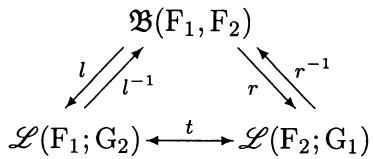
\includegraphics[keepaspectratio]{images/part003_fb3d81cd.jpg}}

其中 t 是转置同构 \(u \mapsto {}^{t}u\) 。鉴于 \(G_{1}\) 与 \(G_{2}\) 上弱拓扑的定义，还可直接看出：当 \(\mathfrak{B}(F_{1}, F_{2})\) 、 \(\mathcal{L}(F_{1}; G_{2})\) 与 \(\mathcal{L}(F_{2}; G_{1})\) 装备逐点收敛拓扑时，前一图中的同构是拓扑向量空间结构之间的同构。

现在设 E 、 F 是两个 Hausdorff 局部凸空间， \(E'\) 、 \(F'\) 是它们的对偶；我们用 \(E_{\sigma}\) 、 \(F_{\sigma}\) 表示装备弱化拓扑 \(\sigma(\mathrm{E}, \mathrm{E}')\) 、 \(\sigma(\mathrm{F}, \mathrm{F}')\) 的空间 E 、 F ，用 \(E_{s}'\) 、 \(F_{s}'\) 表示空间 \(E'\) 、 \(F'\) （装备弱拓扑 \(\sigma(\mathrm{E}', \mathrm{E})\) 、 \(\sigma(\mathrm{F}', \mathrm{F})\) ）。于是，前面的注记在三个空间 \(\mathfrak{B}(\mathrm{E}_{\sigma}, \mathrm{F}_{s}')\) 、 \(\mathcal{L}(\mathrm{E}_{\sigma}; \mathrm{F}_{\sigma})\) 与 \(\mathcal{L}(\mathrm{F}_{s}'; \mathrm{E}_{s}')\) 之间建立了典范同构，也在三个空间 \(\mathfrak{B}(\mathrm{E}_{\sigma}, \mathrm{F}_{\sigma})\) 、 \(\mathcal{L}(\mathrm{E}_{\sigma}; \mathrm{F}_{s}')\) 与 \(\mathcal{L}(\mathrm{F}_{\sigma}; \mathrm{E}_{s}')\) 之间建立了典范同构。我们将注意到， \(\mathfrak{B}(\mathrm{E}_{\sigma}, \mathrm{F}_{\sigma})\) 也等于空间 \(\mathfrak{B}(\mathrm{E}, \mathrm{F})\) ，即 \(E \times F\) 上分别连续双线性型所成的空间（ E 与 F 装备其原来的拓扑），因为 E （相应地， F ）上的每个连续线性形式在 \(E_{\sigma}\) （相应地， \(F_{\sigma}\) ）上连续，反之亦然（TVS, II, §6, No.~1 与 No.~2, 命题 3）。

设 \(\mathcal{B}(\mathrm{E},\mathrm{F})\) 是 \(\mathbf{E}\times \mathbf{F}\) 上连续双线性型所成的空间（ E 与 F 装备其原来的拓扑）；则 \(\mathcal{B}(\mathrm{E},\mathrm{F})\subset \mathfrak{B}(\mathrm{E},\mathrm{F})\) 。

命题 1. --- 双线性型 \(\Phi \in \mathfrak{B}(\mathrm{E},\mathrm{F})\) 属于 \(\mathcal{B}(\mathrm{E},\mathrm{F})\) 的充要条件是：存在 E 的一个 0 的邻域，它在 \(^l\Phi\) 下的像是 \(\mathbf{F}'\) 的一个等度连续子集。

因为，说 \(\Phi\) 连续，意思是存在 E （相应地， F ）中 0 的一个均衡凸邻域 V （相应地， W ），使得 \(|\Phi(x,y)| \leqslant 1\) （对 \(x \in V\) 、 \(y \in W\) ）；这可写成 \(|\langle^{l}\Phi(x), y \rangle| \leqslant 1\) （对 \(x \in V\) 、 \(y \in W\) ），或者写成 \(^{l}\Phi(V) \subset W^{\circ}\) ；由此即得命题，因为考虑到 \(F'\) 的每个等度连续子集都含于 F 中 0 的某个邻域的极集。

推论. --- 若 \(\Phi\) 是 \(\mathbf{E} \times \mathbf{F}\) 上的连续双线性型，则 \(^l\Phi\) 是 \(\mathbf{E}\) 到强对偶 \(\mathbf{F}_b'\) （ \(\mathbf{F}\) 的强对偶）中的连续线性映射。此外，若 \(\mathbf{E}\) 与 \(\mathbf{F}\) 是赋范空间，则 \(\|^l\Phi\| = \| \Phi \|\) 。

第一个断言由命题 1 以及 \(F_{b}^{\prime}\) 中 0 的每个邻域都吸收 \(F^{\prime}\) 的每个等度连续子集这一事实得出。若 E 与 F 赋范，则

\[
\begin{array}{c} \| \Phi \| = \sup _ {\| x \| \leqslant 1, \| y \| \leqslant 1} | \Phi (x, y) | = \sup _ {\| x \| \leqslant 1} \Big (\sup _ {\| y \| \leqslant 1} \big | \langle^ {l} \Phi (x), y \rangle \big | \Big) \\ = \sup _ {\| x \| \leqslant 1} \| ^ {l} \Phi (x) \| = \| ^ {l} \Phi \|, \end{array}
\]

由此得第二个断言。

交换 E 与 F 的角色，对线性映射 \(r\Phi\) 可得到与命题 1 及其推论类似的结果；我们把这些结果的叙述留给读者。

\section{具有性质（GDF）的几类空间}

我们已经知道每个 Fréchet 空间都具有性质（GDF）（TVS, I, §3, No.~3, 定理 1 的推论 5）。

命题 2. --- 设 E 是一个向量空间， \((\mathrm{F}_{\alpha})_{\alpha\in\mathrm{A}}\) 是具有性质（GDF）的局部凸空间的一个族，且对每个 \(\alpha\in A\) ，设 \(h_{\alpha}\) 是 \(F_{\alpha}\) 到 E 中的一个线性映射。若 E 装备使诸 \(h_{\alpha}\) 连续的最细局部凸拓扑，则 E 具有性质（GDF）。

设 \(u\) 是 \(\mathbf{E}\) 到一个 Banach 空间 \(\mathbf{B}\) 中的线性映射，使得在 \(\mathbf{E} \times \mathbf{B}\) 中，图 \(\Gamma\) （ \(u\) 的图）的点的每个收敛序列的每个极限也属于 \(\Gamma\) 。只需证明对每个 \(\alpha \in \mathbf{A}\) ， \(u \circ h_{\alpha}\) 在 \(\mathrm{F}_{\alpha}\) 上连续（TVS, II, §4, No.~4, 命题 5）。现在，设 \((x_n)\) 是 \(\mathrm{F}_{\alpha}\) 的元素的一个序列，具有极限 \(a\) ，且使得序列 \(\left(u(h_{\alpha}(x_n))\right)\) 具有一个极限 \(b \in \mathbf{B}\) 。由于 \(h_{\alpha}\) 连续， \(h_{\alpha}(a)\) 是序列 \((h_{\alpha}(x_n))\) 在 \(\mathbf{E}\) 中的一个极限；因此由假设 \(b = u(h_{\alpha}(a))\) ，且由于 \(\mathrm{F}_{\alpha}\) 具有性质（GDF）， \(u \circ h_{\alpha}\) 连续。

推论. --- 具有性质（GDF）的局部凸空间的每个商空间都具有性质（GDF）。

命题 3. --- 自反 Fréchet 空间的强对偶具有性质（GDF）。

这是命题 2 与下述引理（或 TVS, IV, §3, No.~4, 命题 4）的推论：

引理. --- 设 F 是一个 Fréchet 空间， \(F'\) 是它的强对偶， \(F''\) 是它的双对偶。若 \(F''\) 的每个关于 \(\sigma(F'', F')\) 有界的子集都含于 F 的一个有界子集的闭包（关于 \(\sigma(F'', F')\) ）中，则 \(F'\) 是 Banach 空间的一个序列的直接极限。

因为，设 \((\mathrm{V}_{n})\) 是 F 中 0 的凸、均衡、闭邻域的一个递减的基本序列。对每个整数 n ，设 \(G_{n}\) 是 \(F'\) 的线性子空间，由极集 \(V_{n}^{\circ}\) （ \(V_{n}\) 的极集）生成。在 \(G_{n}\) 中， \(V_{n}^{\circ}\) 是一个吸收性凸集，因此它的度规 \(p_{n}\) 是 \(G_{n}\) 上的一个范数；此外， \(V_{n}^{\circ}\) 是强对偶 \(F'\) 的完备子集（TVS, III, §3, No.~8, 命题 11）；从而 \(G_{n}\) （装备范数 \(p_{n}\) ）是一个 Banach 空间（GT, III, §3, No.~5, 命题 9 的推论 2）。我们将证明 \(F'\) 上的强拓扑是诸 \(G_{n}\) 上这些 Banach 空间拓扑的直接极限，或者等价地说，一个强闭、均衡、凸子集 U （ \(F'\) 的子集）是 0 的强邻域，当且仅当它吸收每个 \(V_{n}^{\circ}\) 。这个条件是必要的，这是显然的；为看出它是充分的，只需证明 U 含有 \(F'\) 的一个桶。事实上，此时它的极集 \(U^{\circ}\) （在 \(F''\) 中）将关于 \(\sigma(\mathrm{F}''\mathrm{,}\mathrm{F}')\) 有界，因而由假设含于 F 的某个有界子集 B 的闭包（关于 \(\sigma(\mathrm{F}''\mathrm{,}\mathrm{F}')\) ）中，由此可以断定 U （它关于 \(\sigma(\mathrm{F}^{\prime},\mathrm{F}''\mathrm{)})\) 是闭的）含有 0 的强邻域 \(B^{\circ}\) （TVS, II, §6, No.~3, 定理 1 与 §8, No.~4）。

由假设，对每个整数 n 存在一个数 \(\lambda_{n}>0\) ，使得 \(\lambda_{n}V_{n}^{\circ}\subset\frac{1}{2}U\) ；设 \(A_{n}\) 是诸 \(\lambda_{i}V_{i}^{\circ}\) （ \(i\leqslant n\) ）的并的凸包。则对每个 n 有 \(A_{n}\subset\frac{1}{2}U\) ；设 W 是诸 \(A_{n}\) 的并； W 是含于 \(\frac{1}{2}U\) 中的一个凸、均衡、吸收集，只需证明它的强闭包（它是一个桶）含于 U 中。

于是，设 \(x'\) 是 \(F'\) 中不属于 U 的一个点。由于每个 \(V_n^\circ\) 关于 \(\sigma(F', F)\) 是紧的，每个 \(A_n\) 亦然（TVS, II, §2, No.~6, 命题 15），且由于 \(x' \notin 2A_n\) ，存在一个元素 \(x_n\) ，它属于 \(A_n\) 在 F 中的极集，使得 \(\langle x', x_n \rangle = 2\) （TVS, II, §5, No.~3, 命题 4）。序列 \((x_n)\) 在 F 中有界：因为每个 \(y' \in F'\) 都属于某个 \(V_k^\circ\) ，于是 \(|\langle y', x_n \rangle| \leqslant \lambda_k^{-1}\) （对 \(n \geqslant k\) ），由此得我们的断言（TVS, IV, §1, No.~1, 命题 1）。设 C 是 F 中包含所有 \(x_n\) 的一个有界、均衡凸集；则 \(C^\circ\) 是 \(F'\) 中 0 的一个邻域，而极集 \(C^{\circ\circ}\) （ \(C^\circ\) 在 \(F''\) 中的极集）关于 \(\sigma(F'', F')\) 是紧的（TVS, III, §3, No.~4, 命题 4 的推论 2 与 No.~5, 命题 7）。于是可以看出，序列 \((x_n)\) 有一个聚点 \(x''\) （在 \(F''\) 中，关于 \(\sigma(F'', F')\) ）；显然 \(\langle x', x'' \rangle = 2\) ，而另一方面， \(x''\) 属于 \(A_n\) 在 \(F''\) 中的极集（对每个 \(n\) ），从而属于极集 \(W^\circ\) （ W 在 \(F''\) 中的极集）。由此得出 \(x' \notin W^{\circ\circ}\) ，因而 x' 不在 W 关于 \(\sigma(F', F'')\) 的闭包中（TVS, II, §6, No.~3, 定理 1 与 §8, No.~4），从而更不在强拓扑的闭包中，证明至此完成。
